% Options for packages loaded elsewhere
\PassOptionsToPackage{unicode}{hyperref}
\PassOptionsToPackage{hyphens}{url}
%
\documentclass[
]{article}
\usepackage{lmodern}
\usepackage{amssymb,amsmath}
\usepackage{ifxetex,ifluatex}
\ifnum 0\ifxetex 1\fi\ifluatex 1\fi=0 % if pdftex
  \usepackage[T1]{fontenc}
  \usepackage[utf8]{inputenc}
  \usepackage{textcomp} % provide euro and other symbols
\else % if luatex or xetex
  \usepackage{unicode-math}
  \defaultfontfeatures{Scale=MatchLowercase}
  \defaultfontfeatures[\rmfamily]{Ligatures=TeX,Scale=1}
\fi
% Use upquote if available, for straight quotes in verbatim environments
\IfFileExists{upquote.sty}{\usepackage{upquote}}{}
\IfFileExists{microtype.sty}{% use microtype if available
  \usepackage[]{microtype}
  \UseMicrotypeSet[protrusion]{basicmath} % disable protrusion for tt fonts
}{}
\makeatletter
\@ifundefined{KOMAClassName}{% if non-KOMA class
  \IfFileExists{parskip.sty}{%
    \usepackage{parskip}
  }{% else
    \setlength{\parindent}{0pt}
    \setlength{\parskip}{6pt plus 2pt minus 1pt}}
}{% if KOMA class
  \KOMAoptions{parskip=half}}
\makeatother
\usepackage{xcolor}
\IfFileExists{xurl.sty}{\usepackage{xurl}}{} % add URL line breaks if available
\IfFileExists{bookmark.sty}{\usepackage{bookmark}}{\usepackage{hyperref}}
\hypersetup{
  pdftitle={lab\_23},
  pdfauthor={Yakovenko Ivan},
  hidelinks,
  pdfcreator={LaTeX via pandoc}}
\urlstyle{same} % disable monospaced font for URLs
\usepackage[margin=1in]{geometry}
\usepackage{color}
\usepackage{fancyvrb}
\newcommand{\VerbBar}{|}
\newcommand{\VERB}{\Verb[commandchars=\\\{\}]}
\DefineVerbatimEnvironment{Highlighting}{Verbatim}{commandchars=\\\{\}}
% Add ',fontsize=\small' for more characters per line
\usepackage{framed}
\definecolor{shadecolor}{RGB}{248,248,248}
\newenvironment{Shaded}{\begin{snugshade}}{\end{snugshade}}
\newcommand{\AlertTok}[1]{\textcolor[rgb]{0.94,0.16,0.16}{#1}}
\newcommand{\AnnotationTok}[1]{\textcolor[rgb]{0.56,0.35,0.01}{\textbf{\textit{#1}}}}
\newcommand{\AttributeTok}[1]{\textcolor[rgb]{0.77,0.63,0.00}{#1}}
\newcommand{\BaseNTok}[1]{\textcolor[rgb]{0.00,0.00,0.81}{#1}}
\newcommand{\BuiltInTok}[1]{#1}
\newcommand{\CharTok}[1]{\textcolor[rgb]{0.31,0.60,0.02}{#1}}
\newcommand{\CommentTok}[1]{\textcolor[rgb]{0.56,0.35,0.01}{\textit{#1}}}
\newcommand{\CommentVarTok}[1]{\textcolor[rgb]{0.56,0.35,0.01}{\textbf{\textit{#1}}}}
\newcommand{\ConstantTok}[1]{\textcolor[rgb]{0.00,0.00,0.00}{#1}}
\newcommand{\ControlFlowTok}[1]{\textcolor[rgb]{0.13,0.29,0.53}{\textbf{#1}}}
\newcommand{\DataTypeTok}[1]{\textcolor[rgb]{0.13,0.29,0.53}{#1}}
\newcommand{\DecValTok}[1]{\textcolor[rgb]{0.00,0.00,0.81}{#1}}
\newcommand{\DocumentationTok}[1]{\textcolor[rgb]{0.56,0.35,0.01}{\textbf{\textit{#1}}}}
\newcommand{\ErrorTok}[1]{\textcolor[rgb]{0.64,0.00,0.00}{\textbf{#1}}}
\newcommand{\ExtensionTok}[1]{#1}
\newcommand{\FloatTok}[1]{\textcolor[rgb]{0.00,0.00,0.81}{#1}}
\newcommand{\FunctionTok}[1]{\textcolor[rgb]{0.00,0.00,0.00}{#1}}
\newcommand{\ImportTok}[1]{#1}
\newcommand{\InformationTok}[1]{\textcolor[rgb]{0.56,0.35,0.01}{\textbf{\textit{#1}}}}
\newcommand{\KeywordTok}[1]{\textcolor[rgb]{0.13,0.29,0.53}{\textbf{#1}}}
\newcommand{\NormalTok}[1]{#1}
\newcommand{\OperatorTok}[1]{\textcolor[rgb]{0.81,0.36,0.00}{\textbf{#1}}}
\newcommand{\OtherTok}[1]{\textcolor[rgb]{0.56,0.35,0.01}{#1}}
\newcommand{\PreprocessorTok}[1]{\textcolor[rgb]{0.56,0.35,0.01}{\textit{#1}}}
\newcommand{\RegionMarkerTok}[1]{#1}
\newcommand{\SpecialCharTok}[1]{\textcolor[rgb]{0.00,0.00,0.00}{#1}}
\newcommand{\SpecialStringTok}[1]{\textcolor[rgb]{0.31,0.60,0.02}{#1}}
\newcommand{\StringTok}[1]{\textcolor[rgb]{0.31,0.60,0.02}{#1}}
\newcommand{\VariableTok}[1]{\textcolor[rgb]{0.00,0.00,0.00}{#1}}
\newcommand{\VerbatimStringTok}[1]{\textcolor[rgb]{0.31,0.60,0.02}{#1}}
\newcommand{\WarningTok}[1]{\textcolor[rgb]{0.56,0.35,0.01}{\textbf{\textit{#1}}}}
\usepackage{graphicx,grffile}
\makeatletter
\def\maxwidth{\ifdim\Gin@nat@width>\linewidth\linewidth\else\Gin@nat@width\fi}
\def\maxheight{\ifdim\Gin@nat@height>\textheight\textheight\else\Gin@nat@height\fi}
\makeatother
% Scale images if necessary, so that they will not overflow the page
% margins by default, and it is still possible to overwrite the defaults
% using explicit options in \includegraphics[width, height, ...]{}
\setkeys{Gin}{width=\maxwidth,height=\maxheight,keepaspectratio}
% Set default figure placement to htbp
\makeatletter
\def\fps@figure{htbp}
\makeatother
\setlength{\emergencystretch}{3em} % prevent overfull lines
\providecommand{\tightlist}{%
  \setlength{\itemsep}{0pt}\setlength{\parskip}{0pt}}
\setcounter{secnumdepth}{-\maxdimen} % remove section numbering

\title{lab\_23}
\author{Yakovenko Ivan}
\date{11/9/2020}

\begin{document}
\maketitle

\hypertarget{data-analysis-in-r}{%
\section{Data Analysis in R}\label{data-analysis-in-r}}

\hypertarget{load-data}{%
\subsection{Load Data}\label{load-data}}

First we need to load our data from file. Let's see what we get:

\begin{Shaded}
\begin{Highlighting}[]
\NormalTok{zipIncome <-}\StringTok{ }\KeywordTok{read.table}\NormalTok{(}\StringTok{'https://hyper.mephi.ru/assets/courseware/v1/94f633ca057a1aa84db0364cf4bfa81d/asset-v1:MEPhIx+CS712DS+2020Fall+type@asset+block/zipIncome.txt'}\NormalTok{, }\DataTypeTok{header =} \OtherTok{TRUE}\NormalTok{, }\DataTypeTok{sep =} \StringTok{'|'}\NormalTok{, }\DataTypeTok{col.names =} \KeywordTok{c}\NormalTok{(}\StringTok{'zipCode'}\NormalTok{, }\StringTok{'income'}\NormalTok{), }\DataTypeTok{comment.char =} \StringTok{"("}\NormalTok{)}

\KeywordTok{head}\NormalTok{(zipIncome, }\DataTypeTok{n =} \DecValTok{10}\NormalTok{)}
\end{Highlighting}
\end{Shaded}

\begin{verbatim}
##    zipCode   income
## 1        0     0.00
## 2        0     0.00
## 3        0     0.00
## 4        0     0.00
## 5        0     0.00
## 6        0 12013.34
## 7        0 15079.26
## 8        0 15626.57
## 9        0 15759.75
## 10       0 15795.29
\end{verbatim}

\hypertarget{analysis}{%
\subsection{Analysis}\label{analysis}}

To find median and mean of average \textbf{income} we use
\texttt{summary()}

\begin{Shaded}
\begin{Highlighting}[]
\NormalTok{tab_summary <-}\StringTok{ }\KeywordTok{summary}\NormalTok{(zipIncome)}
\KeywordTok{cat}\NormalTok{(}\StringTok{"**For income:**"}\NormalTok{, tab_summary[,}\DecValTok{2}\NormalTok{], }\DataTypeTok{sep=}\StringTok{"}\CharTok{\textbackslash{}n}\StringTok{"}\NormalTok{)}
\end{Highlighting}
\end{Shaded}

\textbf{For income:} Min. : 0\\
1st Qu.: 37644\\
Median : 44163\\
Mean : 48245\\
3rd Qu.: 54373\\
Max. :250000

Let's look at a scatter plot of data. Outlier values are \(\$0\) and
\(\$250000\)

\begin{Shaded}
\begin{Highlighting}[]
\KeywordTok{plot}\NormalTok{(zipIncome)}
\end{Highlighting}
\end{Shaded}

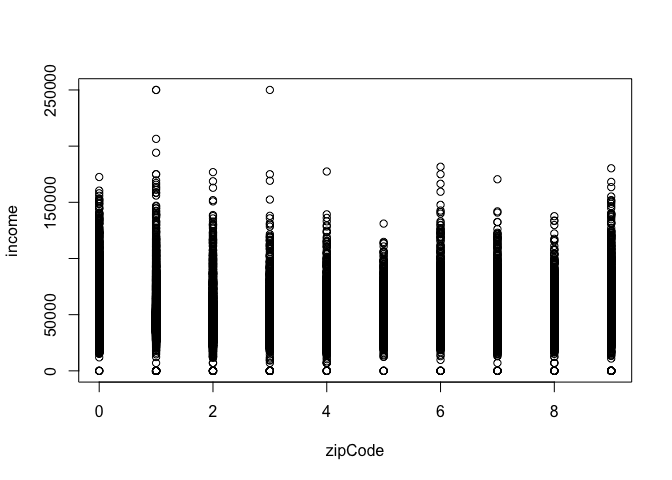
\includegraphics{lab23_files/figure-latex/unnamed-chunk-3-1.pdf}

To avoid outliers let's create subset of data where
\(\$7,000 < income < \$200,000\) and build a simple boxplot:

\begin{Shaded}
\begin{Highlighting}[]
\NormalTok{subset_data <-}\StringTok{ }\KeywordTok{subset}\NormalTok{(zipIncome, income}\OperatorTok{>}\DecValTok{7000} \OperatorTok{&}\StringTok{ }\NormalTok{income }\OperatorTok{<}\StringTok{ }\DecValTok{200000}\NormalTok{)}
\NormalTok{tab_subset <-}\StringTok{ }\KeywordTok{summary}\NormalTok{(subset_data)}
\KeywordTok{cat}\NormalTok{(}\StringTok{"**For income:**"}\NormalTok{, tab_subset[,}\DecValTok{2}\NormalTok{], }\DataTypeTok{sep=}\StringTok{"}\CharTok{\textbackslash{}n}\StringTok{"}\NormalTok{)}
\end{Highlighting}
\end{Shaded}

\begin{verbatim}
## **For income:**
## Min.   :  8465  
## 1st Qu.: 37755  
## Median : 44234  
## Mean   : 48465  
## 3rd Qu.: 54444  
## Max.   :194135
\end{verbatim}

\begin{Shaded}
\begin{Highlighting}[]
\KeywordTok{boxplot}\NormalTok{(}\DataTypeTok{formula=}\NormalTok{income }\OperatorTok{~}\StringTok{ }\NormalTok{zipCode, }\DataTypeTok{col=}\StringTok{"white"}\NormalTok{, }\DataTypeTok{data =}\NormalTok{ subset_data, }\DataTypeTok{main =} \StringTok{'Average Household Income by Zip Code'}\NormalTok{, }\DataTypeTok{xlab =} \StringTok{'Zip Code'}\NormalTok{, }\DataTypeTok{ylab =} \StringTok{'Income'}\NormalTok{)}
\end{Highlighting}
\end{Shaded}

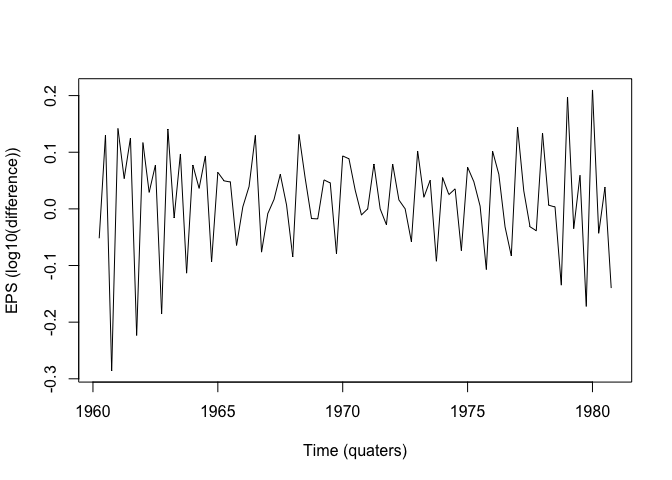
\includegraphics{lab23_files/figure-latex/unnamed-chunk-5-1.pdf}

\textbf{Or with log scale over Y}

\begin{Shaded}
\begin{Highlighting}[]
\KeywordTok{boxplot}\NormalTok{(income }\OperatorTok{~}\StringTok{ }\NormalTok{zipCode, }\DataTypeTok{col=}\StringTok{"white"}\NormalTok{, }\DataTypeTok{data =}\NormalTok{ subset_data, }\DataTypeTok{main =} \StringTok{'Average Household Income by Zip Code'}\NormalTok{, }\DataTypeTok{xlab =} \StringTok{'Zip Code'}\NormalTok{, }\DataTypeTok{ylab =} \StringTok{'Income'}\NormalTok{, }\DataTypeTok{log =} \StringTok{'y'}\NormalTok{)}
\end{Highlighting}
\end{Shaded}

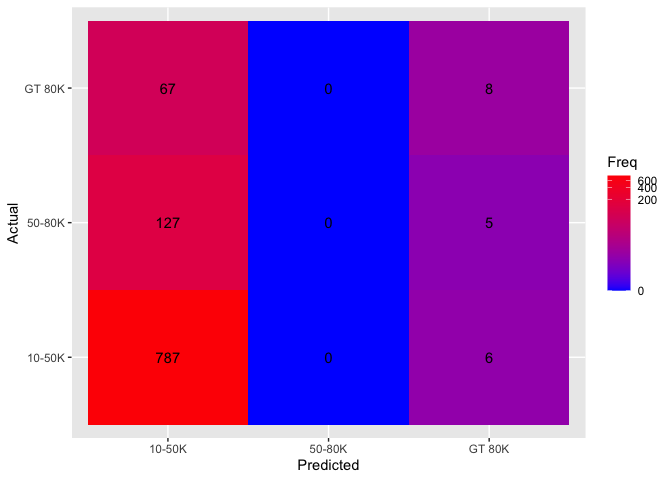
\includegraphics{lab23_files/figure-latex/unnamed-chunk-6-1.pdf}

For the next step we are needed in \textbf{ggplot2} package. Let's check
it and install if it is necessary.

\begin{Shaded}
\begin{Highlighting}[]
 \ControlFlowTok{if}\NormalTok{ (}\OperatorTok{!}\KeywordTok{require}\NormalTok{(}\StringTok{'ggplot2'}\NormalTok{))}
\NormalTok{   \{}
      \KeywordTok{install.packages}\NormalTok{(}\StringTok{'ggplot2'}\NormalTok{, }\DataTypeTok{dependencies =} \OtherTok{TRUE}\NormalTok{)}
      \KeywordTok{library}\NormalTok{(}\StringTok{'ggplot2'}\NormalTok{)}
\NormalTok{   \}}
\end{Highlighting}
\end{Shaded}

\begin{verbatim}
## Loading required package: ggplot2
\end{verbatim}

\hypertarget{making-plots-with-ggplot2}{%
\subsubsection{Making plots with
ggplot2}\label{making-plots-with-ggplot2}}

\begin{Shaded}
\begin{Highlighting}[]
\NormalTok{plt <-}\StringTok{ }\KeywordTok{ggplot}\NormalTok{(}\DataTypeTok{data=}\NormalTok{subset_data, }\KeywordTok{aes}\NormalTok{(}\KeywordTok{as.factor}\NormalTok{(zipCode), income))}
\NormalTok{plt }\OperatorTok{+}\StringTok{ }\KeywordTok{geom_point}\NormalTok{(}\DataTypeTok{position=}\StringTok{'jitter'}\NormalTok{, }\DataTypeTok{alpha=}\FloatTok{0.2}\NormalTok{) }\OperatorTok{+}\StringTok{ }\KeywordTok{scale_y_log10}\NormalTok{()}
\end{Highlighting}
\end{Shaded}

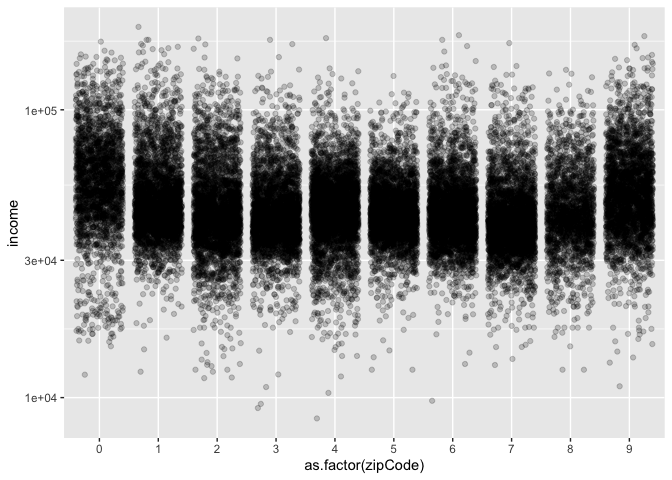
\includegraphics{lab23_files/figure-latex/unnamed-chunk-8-1.pdf}

And colorful ggplot:

\begin{Shaded}
\begin{Highlighting}[]
\NormalTok{color_plt <-}\StringTok{ }\KeywordTok{ggplot}\NormalTok{(}\DataTypeTok{data=}\NormalTok{subset_data, }\KeywordTok{aes}\NormalTok{(}\KeywordTok{as.factor}\NormalTok{(zipCode), income))}
\NormalTok{color_plt <-}\StringTok{ }\NormalTok{color_plt }\OperatorTok{+}\StringTok{ }\KeywordTok{geom_point}\NormalTok{(}\KeywordTok{aes}\NormalTok{(}\DataTypeTok{color=}\KeywordTok{factor}\NormalTok{(zipCode)), }\DataTypeTok{position=}\StringTok{'jitter'}\NormalTok{, }\DataTypeTok{alpha=}\FloatTok{0.2}\NormalTok{) }\OperatorTok{+}\StringTok{ }\KeywordTok{scale_y_log10}\NormalTok{()}
\NormalTok{color_plt <-}\StringTok{ }\NormalTok{color_plt }\OperatorTok{+}\StringTok{ }\KeywordTok{geom_boxplot}\NormalTok{(}\KeywordTok{aes}\NormalTok{(}\DataTypeTok{group=}\NormalTok{zipCode), }\DataTypeTok{alpha =} \FloatTok{0.1}\NormalTok{, }\DataTypeTok{outlier.size =} \OperatorTok{-}\OtherTok{Inf}\NormalTok{)}
\KeywordTok{plot}\NormalTok{(color_plt }\OperatorTok{+}\StringTok{ }\KeywordTok{labs}\NormalTok{(}\DataTypeTok{title =} \StringTok{'Average Household Income by Zip Code'}\NormalTok{, }\DataTypeTok{x =} \StringTok{'Zip Code'}\NormalTok{, }\DataTypeTok{y =} \StringTok{'Income'}\NormalTok{, }\DataTypeTok{color =} \StringTok{'Region'}\NormalTok{))}
\end{Highlighting}
\end{Shaded}

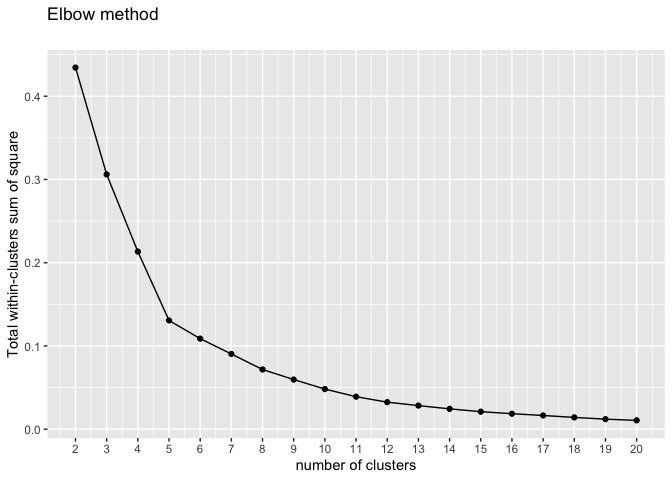
\includegraphics{lab23_files/figure-latex/unnamed-chunk-9-1.pdf}

\hypertarget{conclusion}{%
\subsection{Conclusion}\label{conclusion}}

After basic analysis of this data we can say that 0 and 9 zip codes have
the largest average income.

\end{document}
